% Provenance (never printed): see sources/outline_sources.md (Year 2: field and laboratory methods ---
% igneous and metamorphic petrography, chemical analysis by XRF, ICP-MS and microprobe, isotope mass
% spectrometry, a mapping campaign). Modelled on Book 3 ch. 6.
% Textures: BGS RR 99-02 (Robertson 1999), Open University Virtual Microscope, Carleton BH250,
% UCSB Geology 102C (Hacker); QAPF: BGS RR 99-06 (Gillespie and Styles 1999); instruments: SERC
% Geochemical Instrumentation and Analysis sheets (EPMA, WDS, XRF, TIMS, MC-ICPMS); XRF procedure
% and reference-material results: USGS OFR 02-223 and its chapter T (Taggart and Siems 2002); Sr
% isotopes: CIAAW; spike and mass bias: Cheong, Jeong and Kwon (2014). Ledger rows in
% sources/ledger/book4.md; curves and stations from figdata/bachelor-2/labmethods.py, numbers from
% the Book 4 second-writer scratch calculator calc/ch31.py. Observation only: the professional work
% is described in the third person.
\chapter{Veldwerk- en laboratoriummethoden II}\label{ch:b2:field-lab-methods-2}

Elk getal in de petrologiehoofdstukken van dit boek begon als een gesteente in een zak, een slijpplaatje onder een
microscoop en een poeder in een instrument. Een mineraalsamenstelling uitgezet in een fasediagram, het
silicagehalte dat een lava een naam geeft, de strontiumisotopenverhouding die een mantelbron opspoort: elk
kwam uit een keten van handelingen die bij een ontsluiting begon, en elk draagt de fouten van elke
schakel. Dit hoofdstuk volgt die keten voor de gesteenten van de sokkel van de Varden Hills: texturen lezen
in slijpplaatjes, mineralen tellen, het hele gesteente analyseren, daarna afzonderlijke mineralen, daarna isotopen,
en bij elke stap vragen hoe goed het getal is.

\begin{recall}
\textbf{Uit Boek~3}: veldstation, veldboek, georiënteerd monster, dunne slijpplaat,
polariserende microscoop, vlakgepolariseerd licht, gekruiste polarisatoren; optische identificatie van de gesteentevormende
mineralen; herberekening van een mineraalformule uit een oxideanalyse op een vast aantal zuurstofatomen,
en van driewaardig ijzer via de ladingsbalans; foliatie en schistositeit; isochroon, beginverhouding en de
kleinste-kwadratenlijn. \textbf{Uit de scheikundeboeken}: massaspectrometrie, inductief gekoppeld plasma;
kalibratiecurve, detectiegrens, bepalingsgrens, precisie, juistheid, systematische afwijking,
herhaalbaarheid, standaardafwijking van het gemiddelde. \textbf{Uit de natuurkundeboeken}: karakteristieke röntgenstraling
en de wet van Moseley; de wet van Bragg; oppervlaktespanning; voortplanting van onzekerheden.
\textbf{Uit de wiskundeboeken}: binomiale verdeling, haar gemiddelde en variantie.
\textbf{Uit \cref{ch:b2:magmatic-series}}: \omterm{def:b2:magmatic-series:qapf}{modale samenstelling}, \omterm{def:b2:magmatic-series:qapf}{QAPF-diagram}.
\textbf{Uit \cref{ch:b2:isotope-geochemistry}}: \omterm{def:b2:isotope-geochemistry:tracer}{radiogene isotopentracer}, \omterm{def:b2:isotope-geochemistry:standards}{isotopische referentiestandaard}.
\end{recall}

\section{Petrografie: texturen als geschiedenis}\label{sec:b2:field-lab-methods-2:petrography}

Boek~3 gebruikte de polariserende microscoop om mineralen te identificeren. Een petrograaf leest ook
hoe de korrels zijn gerangschikt, omdat die rangschikking de volgorde vastlegt waarin ze groeiden. Twee
texturen zijn de meest voorkomende getuigen van kristallisatie uit een smelt en van herkristallisatie in
vaste toestand.

\begin{definition}[Ofitische textuur, granoblastische textuur]\label{def:b2:field-lab-methods-2:textures}
Een stollingsgesteente heeft een \emph{ofitische textuur}\index{ofitische textuur} wanneer grote pyroxeenkristallen
kleine, willekeurig georiënteerde latten plagioklaas omsluiten; de textuur is typisch voor doleriet, gabbro
en basalt. Een metamorf gesteente heeft een \emph{granoblastische textuur}\index{granoblastische textuur} wanneer het
een aggregaat is van ruwweg isometrische kristallen van ongeveer dezelfde grootte, vaak xenomorf,
waarvan de rechte grenzen per drie samenkomen onder hoeken van bijna \ang{120}.
\end{definition}
% ledger: carletonB:ophitic, ouVM:textures, bgsM:textures

In een ofitisch gesteente zijn de omsloten latten heel en idiomorf, en vult het pyroxeen de ruimte
ertussen: het plagioklaas groeide eerst, het pyroxeen eromheen. De hoeken van \ang{120} van een
\omterm{def:b2:field-lab-methods-2:textures}{granoblastische textuur} zijn die van korrels die de tijd hebben gehad om hun grenzen aan te passen; petrografisch lesmateriaal leest zulke
tripelpunten als een teken van chemisch en textureel evenwicht. De hoek volgt uit een evenwicht van krachten, waarbij de korrelgrenzen aan hun
gemeenschappelijke lijn trekken zoals zeepvliezen (oppervlaktespanning, uit de natuurkundeboeken).
% ledger: ouVM:equilibrium

\begin{proposition}[Hoeken in een tripelpunt]\label{prop:b2:field-lab-methods-2:triple}
Laat drie korrelgrenzen samenkomen langs een lijn, met spanningen (energieën per oppervlakte-eenheid) $\gamma_1$,
$\gamma_2$, $\gamma_3$, en zij $\theta_i$ de hoek tussen de twee andere grenzen dan
grens $i$. In evenwicht geldt
\begin{equation}
\frac{\gamma_1}{\sin\theta_1} = \frac{\gamma_2}{\sin\theta_2} = \frac{\gamma_3}{\sin\theta_3},
\label{eq:b2:field-lab-methods-2:lami}
\end{equation}
en drie gelijke spanningen komen samen onder drie hoeken van \ang{120}.
\end{proposition}

\begin{proof}
In een vlak loodrecht op het tripelpunt trekt elke grens het tripelpunt langs haar eigen spoor
met de kracht $\gamma_i$ per lengte-eenheid. In evenwicht is de som van de drie krachten nul, zodat ze, kop aan
staart geplaatst, een driehoek sluiten. De hoek van de driehoek tegenover de zijde $\gamma_i$ is
$\pi - \theta_i$, met als sinus $\sin\theta_i$, en de sinusregel in de driehoek geeft
\eqref{eq:b2:field-lab-methods-2:lami}. Als de drie spanningen gelijk zijn, is de driehoek
gelijkzijdig, en is elke buitenhoek $\theta_i$ gelijk aan $\pi - \pi/3 = 2\pi/3$, dat is \ang{120}.
\end{proof}

\begin{omfigure}
\centering
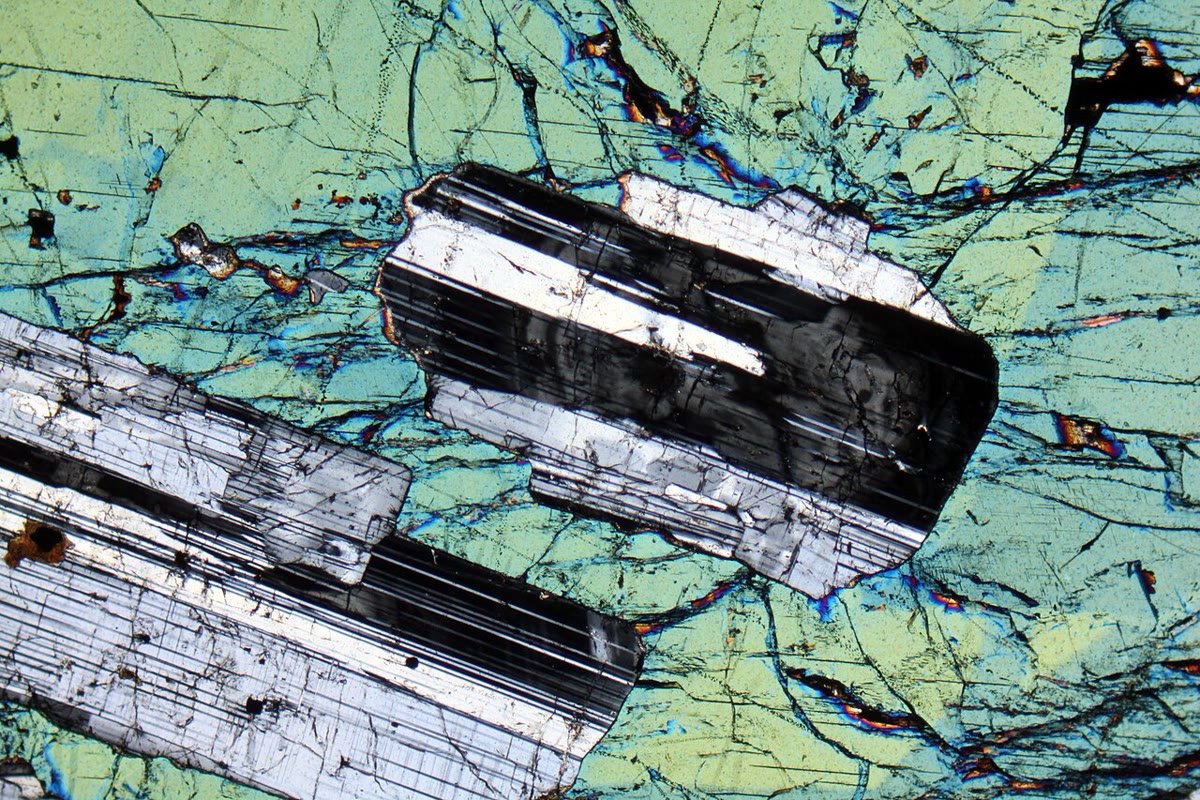
\includegraphics[height=4.6cm]{images/book4/b2-31-ophitic.jpg}\quad
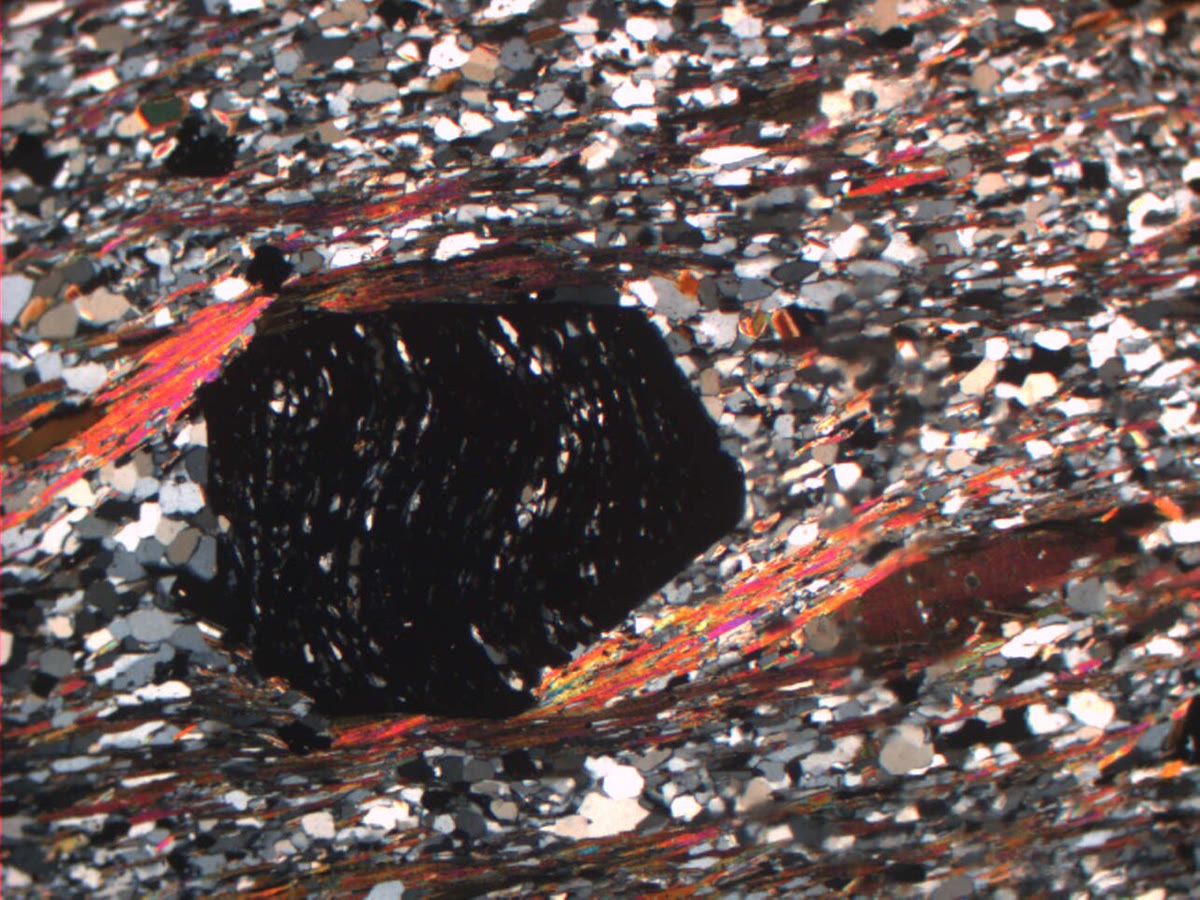
\includegraphics[height=4.6cm]{images/book4/b2-31-garnet-porphyroblast.jpg}
\par\smallskip{\small Twee texturen tussen gekruiste polarisatoren. Links: één kristal augiet (blauw
en groen) omsluit latten plagioklaas die door hun tweelingvorming gestreept zijn, de rangschikking van een \omterm{def:b2:field-lab-methods-2:textures}{ofitische
textuur}; beeldveld \qty{7}{mm}. Foto Strekeisen, CC BY-SA 4.0 (Wikimedia Commons).
Rechts: een granaat--glimmerschist. De granaat, zwart omdat hij isotroop is, is een groot kristal dat
in vaste toestand groeide; insluitsels van kwarts doorkruisen hem in sporen, en de foliatie van muscoviet
(heldere kleuren), biotiet (bruin) en kwarts (grijs) buigt eromheen. Foto Jackdann88,
CC BY 3.0 (Wikimedia Commons).}
\end{omfigure}
% ledger: photo:b2-31-ophitic, photo:b2-31-garnet

Metamorfe mineralen groeien niet allemaal even snel. Sommige soorten overgroeien de andere tot zeer grote kristallen,
die de kleine korrels eromheen opslokken terwijl ze groeien.

\begin{definition}[Porfiroblast, poikiloblast, insluitselspoor, corona]\label{def:b2:field-lab-methods-2:porphyroblast}
Een \emph{porfiroblast}\index{porfiroblast} is een groot kristal dat tijdens de \omterm{def:b2:metamorphic-facies:metamorphism}{metamorfose} groeide
in een fijnkorreliger grondmassa; granaat, stauroliet, cordieriet en chloritoïd vormen ze, van
millimeters tot verscheidene centimeters groot. Een \emph{poikiloblast}\index{poikiloblast} is een
porfiroblast die veel insluitsels van andere mineralen bevat. Een
\emph{insluitselspoor}\index{insluitselspoor} is een rij gerichte insluitsels in een porfiroblast, die
het maaksel van de grondmassa bewaart van het moment waarop het kristal haar overgroeide. Een
\emph{corona}\index{corona (reactietextuur)} is een rand van een of meer nieuwe mineralen die een mineraal dat aan het
afbreken was volledig omringt, omdat dat mineraal niet langer stabiel was met zijn
buren: een reactietextuur, bevroren voordat de reactie voltooid was.
\end{definition}
% ledger: bgsM:textures, ouVM:textures

Het vergelijken van het \omterm{def:b2:field-lab-methods-2:porphyroblast}{insluitselspoor} ($S_i$, het interne maaksel) met de foliatie buiten het kristal
($S_e$, het externe maaksel) dateert de groei van een \omterm{def:b2:field-lab-methods-2:porphyroblast}{porfiroblast} ten opzichte van de deformatie die
de foliatie maakte. De criteria hieronder, getekend in de figuur, zijn die van gangbaar lesmateriaal.
% ledger: ucsbH:inclusion-trails

\begin{method}[De groei van een porfiroblast dateren uit zijn insluitselsporen]\label{met:b2:field-lab-methods-2:timing}
Zoek een doorsnede loodrecht op de foliatie en vergelijk dan $S_i$ en $S_e$.
\begin{enumerate}
  \item \textbf{Willekeurige insluitsels}, $S_e$ om het kristal afgebogen: het groeide voordat de
        foliatie ontstond (\emph{pretektonisch}).
  \item \textbf{Recht $S_i$, afgesneden aan de rand}, niet doorlopend met een afgebogen $S_e$: het groeide
        over een oudere foliatie heen, tussen twee deformaties (\emph{intertektonisch}).
  \item \textbf{Gebogen $S_i$}, doorlopend met $S_e$: het groeide terwijl de foliatie ontstond, en roteerde
        of werd overgroeid terwijl het groeide (\emph{syntektonisch}; de spiraal van een sneeuwbalgranaat).
  \item \textbf{Recht $S_i$, doorlopend met een niet-afgebogen $S_e$}: het groeide na de foliatie
        (\emph{posttektonisch}).
\end{enumerate}
\end{method}

\begin{omfigure}
\centering
\begin{tikzpicture}[x=1cm, y=1cm, font=\scriptsize]
% schematic after the criteria of ledger ucsbH:inclusion-trails
% panel 1: pre-tectonic
\begin{scope}[shift={(0,0)}]
\draw[omExo, line width=0.5pt] (-1.5,0.95) .. controls (-0.6,0.95) and (-0.5,0.85) .. (0,0.85) .. controls (0.5,0.85) and (0.6,0.95) .. (1.5,0.95);
\draw[omExo, line width=0.5pt] (-1.5,-0.95) .. controls (-0.6,-0.95) and (-0.5,-0.85) .. (0,-0.85) .. controls (0.5,-0.85) and (0.6,-0.95) .. (1.5,-0.95);
\draw[omExo, line width=0.5pt] (-1.5,0.45) .. controls (-0.9,0.45) and (-0.85,0.78) .. (0,0.78) .. controls (0.85,0.78) and (0.9,0.45) .. (1.5,0.45);
\draw[omExo, line width=0.5pt] (-1.5,-0.45) .. controls (-0.9,-0.45) and (-0.85,-0.78) .. (0,-0.78) .. controls (0.85,-0.78) and (0.9,-0.45) .. (1.5,-0.45);
\draw[omExo, line width=0.5pt] (-1.5,0) -- (-0.78,0); \draw[omExo, line width=0.5pt] (0.78,0) -- (1.5,0);
\filldraw[fill=omThm!15, draw=omThm, line width=0.6pt] (0,0) circle (0.72);
\draw[black, line width=0.7pt] (-0.4,0.2) -- (-0.25,0.35); \draw[black, line width=0.7pt] (0.1,0.35) -- (0.3,0.2);
\draw[black, line width=0.7pt] (-0.35,-0.2) -- (-0.15,-0.25); \draw[black, line width=0.7pt] (0.2,-0.15) -- (0.25,-0.4);
\draw[black, line width=0.7pt] (-0.05,0.05) -- (0.05,-0.1); \draw[black, line width=0.7pt] (0.35,0.0) -- (0.5,0.12);
\node at (0,-1.3) {pretektonisch};
\end{scope}
% panel 2: inter-tectonic
\begin{scope}[shift={(3.4,0)}]
\draw[omExo, line width=0.5pt] (-1.5,0.95) .. controls (-0.6,0.95) and (-0.5,0.85) .. (0,0.85) .. controls (0.5,0.85) and (0.6,0.95) .. (1.5,0.95);
\draw[omExo, line width=0.5pt] (-1.5,-0.95) .. controls (-0.6,-0.95) and (-0.5,-0.85) .. (0,-0.85) .. controls (0.5,-0.85) and (0.6,-0.95) .. (1.5,-0.95);
\draw[omExo, line width=0.5pt] (-1.5,0.45) .. controls (-0.9,0.45) and (-0.85,0.78) .. (0,0.78) .. controls (0.85,0.78) and (0.9,0.45) .. (1.5,0.45);
\draw[omExo, line width=0.5pt] (-1.5,-0.45) .. controls (-0.9,-0.45) and (-0.85,-0.78) .. (0,-0.78) .. controls (0.85,-0.78) and (0.9,-0.45) .. (1.5,-0.45);
\draw[omExo, line width=0.5pt] (-1.5,0) -- (-0.78,0); \draw[omExo, line width=0.5pt] (0.78,0) -- (1.5,0);
\filldraw[fill=omThm!15, draw=omThm, line width=0.6pt] (0,0) circle (0.72);
\begin{scope}
\clip (0,0) circle (0.66);
\foreach \k in {-0.6,-0.3,0,0.3,0.6} {\draw[black, line width=0.7pt, dash pattern=on 2pt off 1.5pt] (-0.8,\k-0.45) -- (0.8,\k+0.45);}
\end{scope}
\node at (0,-1.3) {intertektonisch};
\end{scope}
% panel 3: syn-tectonic
\begin{scope}[shift={(6.8,0)}]
\draw[omExo, line width=0.5pt] (-1.5,0.8) -- (1.5,0.8);
\draw[omExo, line width=0.5pt] (-1.5,-0.8) -- (1.5,-0.8);
\draw[omExo, line width=0.5pt] (-1.5,0.4) -- (-0.6,0.4); \draw[omExo, line width=0.5pt] (0.6,0.4) -- (1.5,0.4);
\draw[omExo, line width=0.5pt] (-1.5,0) -- (-0.72,0); \draw[omExo, line width=0.5pt] (0.72,0) -- (1.5,0);
\draw[omExo, line width=0.5pt] (-1.5,-0.4) -- (-0.6,-0.4); \draw[omExo, line width=0.5pt] (0.6,-0.4) -- (1.5,-0.4);
\filldraw[fill=omThm!15, draw=omThm, line width=0.6pt] (0,0) circle (0.72);
\draw[black, line width=0.7pt, dash pattern=on 2pt off 1.5pt] (-0.6,0.4) .. controls (-0.35,0.4) and (-0.2,0.3) .. (-0.05,0.4) .. controls (0.1,0.5) and (0.35,0.4) .. (0.6,0.4);
\draw[black, line width=0.7pt, dash pattern=on 2pt off 1.5pt] (-0.72,0) .. controls (-0.3,0) and (-0.3,-0.45) .. (0,0) .. controls (0.3,0.45) and (0.3,0) .. (0.72,0);
\draw[black, line width=0.7pt, dash pattern=on 2pt off 1.5pt] (-0.6,-0.4) .. controls (-0.35,-0.4) and (-0.1,-0.5) .. (0.05,-0.4) .. controls (0.2,-0.3) and (0.35,-0.4) .. (0.6,-0.4);
\node at (0,-1.3) {syntektonisch};
\end{scope}
% panel 4: post-tectonic
\begin{scope}[shift={(10.2,0)}]
\foreach \k in {-0.8,-0.4,0,0.4,0.8} {\draw[omExo, line width=0.5pt] (-1.5,\k) -- (1.5,\k);}
\filldraw[fill=omThm!15, draw=omThm, line width=0.6pt] (0,0) circle (0.72);
\begin{scope}
\clip (0,0) circle (0.66);
\foreach \k in {-0.8,-0.4,0,0.4,0.8} {\draw[black, line width=0.7pt, dash pattern=on 2pt off 1.5pt] (-0.8,\k) -- (0.8,\k);}
\end{scope}
\node at (0,-1.3) {posttektonisch};
\end{scope}
\end{tikzpicture}
\par\smallskip{\small Insluitselsporen (zwart, gestreept) in een \omterm{def:b2:field-lab-methods-2:porphyroblast}{porfiroblast} (rood) en de foliatie
erbuiten (grijs), in doorsneden loodrecht op de foliatie (schematisch). Van links naar rechts:
insluitsels gegroeid vóór de foliatie, die om het kristal heen buigt; een recht ouder maaksel, afgesneden
aan de rand; een spoor dat in de foliatie overbuigt, omdat het kristal tijdens de groei roteerde; een
recht spoor dat de ongestoorde foliatie voortzet.}
\end{omfigure}

Petrografie is ook kwantitatief. De verhoudingen van de mineralen van een grofkorrelig stollingsgesteente
geven het een naam in het \omterm{def:b2:magmatic-series:qapf}{QAPF-diagram} (\cref{ch:b2:magmatic-series}), en ze worden onder de
microscoop gemeten.

\begin{definition}[Modale analyse, puntentelling]\label{def:b2:field-lab-methods-2:modal}
Een \emph{modale analyse}\index{modale analyse} is de meting van de \omterm{def:b2:magmatic-series:qapf}{modale samenstelling} van een
gesteente. Bij \emph{puntentelling}\index{puntentelling} wordt een
slijpplaatje in gelijke stappen langs een regelmatig raster onder het dradenkruis van de microscoop verschoven, en wordt
het mineraal onder het dradenkruis op elk punt genoteerd; het aandeel van de punten dat
op een mineraal valt, schat het aandeel ervan in het gesteente.
\end{definition}

\begin{proposition}[Wat puntentelling meet, en hoe goed]\label{prop:b2:field-lab-methods-2:counting}
(a) In een gesteente zonder voorkeursoriëntatie heeft de oppervlaktefractie van een mineraal in een willekeurig geplaatste doorsnede
gemiddeld de waarde van zijn volumefractie. (b) Als $n$ punten onafhankelijk vallen
op een mineraal met oppervlaktefractie $p$, heeft het getelde aandeel $\hat p = k/n$ gemiddelde $p$ en
standaardafwijking
\begin{equation}
\sigma = \sqrt{\frac{p(1-p)}{n}} , \qquad\text{zodat}\qquad n = \frac{p(1-p)}{\sigma^2}
\label{eq:b2:field-lab-methods-2:binomial}
\end{equation}
punten nodig om een standaardafwijking $\sigma$ te bereiken.
\end{proposition}

\begin{proof}
(a) Snijd een blok gesteente met hoogte $H$ in evenwijdige doorsneden met oppervlakte $S$. Het volume van het
mineraal is $\int_0^H a(z)\,\mathrm{d}z$, waarbij $a(z)$ zijn oppervlakte is in de doorsnede op hoogte $z$;
na deling door het volume $SH$ is de volumefractie het gemiddelde van de oppervlaktefractie $a(z)/S$ over
alle hoogten, wat de verwachtingswaarde is voor een willekeurig gekozen hoogte. (b) Elk punt valt met kans $p$ op het
mineraal, onafhankelijk van de andere, zodat het aantal treffers $k$ de
binomiale verdeling met parameters $n$ en $p$ volgt, met gemiddelde $np$ en variantie $np(1-p)$. Delen door
$n$ geeft het gemiddelde $p$ en de variantie $p(1-p)/n$ van $\hat p$.
\end{proof}

Het bewijs van (b) veronderstelt onafhankelijke punten, wat een rasterstap groter dan de korrels
benadert. Voor een mineraal dat \qty{30}{\percent} van een gesteente uitmaakt, geven 500 punten $\sigma =
\sqrt{0.3 \times 0.7/500} = 0.020$, twee procentpunten; één procentpunt bereiken vraagt
$0.21/0.01^2 = 2100$ punten, vier keer zoveel, omdat $\sigma$ slechts daalt als $1/\sqrt n$. De
relatieve fout, $\sigma/p = \sqrt{(1-p)/(np)}$, is het grootst voor de zeldzame mineralen (figuur hieronder,
links). De getelde verhoudingen worden daarna herberekend om het gesteente te benoemen: een modus met
\qty{10}{\percent} kwarts, 30 alkaliveldspaat, 20 plagioklaas en 40 mafische mineralen geeft voor Q, A en
P 16.7, 50.0 en 33.3 zodra de drie felsische componenten op een som van 100 zijn gebracht. In de
QAP-driehoek is een gesteente met Q tussen 20 en 60 een graniet wanneer zijn verhouding P/(A+P) tussen 10 en
\qty{65}{\percent} ligt: een syenograniet onder 35, een monzograniet erboven; van 65 tot 90 is het een
granodioriet, boven 90 een tonaliet. De kleurindex $M'$ is het aandeel donkere mineralen, dat
wil zeggen de mafische en verwante mineralen behalve muscoviet, apatiet en primair carbonaat; een gesteente is
leucocraat onder 35, mesocraat van 35 tot 65, melanocraat van 65 tot 90.
% ledger: bgsI:qapf, bgsI:colour-index

\begin{omfigure}
\centering
\begin{minipage}[b]{0.49\linewidth}\centering
\begin{tikzpicture}
\begin{axis}[omrecord, width=0.96\linewidth, height=5.0cm, xmode=log, xmin=100, xmax=3000,
  ymin=0, ymax=45, xlabel={getelde punten, $n$}, ylabel={relatieve fout $\sigma/p$ (\unit{\percent})},
  xtick={100,300,1000,3000}, xticklabels={100,300,1000,3000}, log ticks with fixed point,
  tick label style={font=\scriptsize}, label style={font=\small}]
% computed in figdata/bachelor-2/labmethods.py part pc (binomial counting)
\addplot[omThm, line width=1.1pt] table[x=n, y=rel05] {figdata/out/bachelor-2-labmethods-pc.dat};
\addplot[omProp, line width=1.1pt] table[x=n, y=rel20] {figdata/out/bachelor-2-labmethods-pc.dat};
\addplot[omDef, line width=1.1pt] table[x=n, y=rel50] {figdata/out/bachelor-2-labmethods-pc.dat};
\node[font=\scriptsize, text=omThm, anchor=south west] at (axis cs:330,24) {$p = 0.05$};
\node[font=\scriptsize, text=omProp, anchor=south west] at (axis cs:104,21.5) {$p = 0.2$};
\node[font=\scriptsize, text=omDef, anchor=south west] at (axis cs:104,10.3) {$p = 0.5$};
\end{axis}
\end{tikzpicture}
\end{minipage}\hfill
\begin{minipage}[b]{0.49\linewidth}\centering
\begin{tikzpicture}
\begin{axis}[omrecord, width=0.96\linewidth, height=5.0cm, xmin=52, xmax=76, ymin=-1.0, ymax=0.75,
  xlabel={aanbevolen \ce{SiO2} (\unit{\percent})}, ylabel={verschil (\unit{\percent})},
  tick label style={font=\scriptsize}, label style={font=\small},
  ytick={-0.8,-0.4,0,0.4}, yticklabel style={/pgf/number format/fixed}]
% data: figdata/bachelor-2/labmethods.py part xrf; ledger: usgsT:sio2-table
\addplot[black!40, densely dotted] coordinates {(52,0) (76,0)};
\addplot[only marks, mark=*, mark size=1.5pt, omDef, error bars/.cd, y dir=both, y explicit]
  table[x=rec, y=diff, y error=s] {figdata/out/bachelor-2-labmethods-xrf.dat};
\node[font=\scriptsize, anchor=east] at (axis cs:73.0,-0.62) {RGM-1};
\node[font=\scriptsize, anchor=west] at (axis cs:56.6,0.40) {JA-2};
\node[font=\scriptsize, anchor=west] at (axis cs:60.8,-0.55) {AMH-1};
\node[font=\scriptsize, anchor=north] at (axis cs:54.1,-0.10) {BCR-2};
\end{axis}
\end{tikzpicture}
\end{minipage}
\par\smallskip{\small Links: relatieve standaardfout van een modaal aandeel $p$ gemeten door
\omterm{def:b2:field-lab-methods-2:modal}{puntentelling}, \eqref{eq:b2:field-lab-methods-2:binomial}, voor een zeldzaam, een gewoon en een overvloedig mineraal.
Rechts: juistheid van silica door röntgenfluorescentie op \omterm{def:b2:field-lab-methods-2:xrf}{gesmolten tabletten} voor tien referentiematerialen van gesteenten,
van basalt tot graniet; elke stip is het gemiddelde van 2 tot 30 analyses min de aanbevolen waarde, met
de standaardafwijking van de analyses als balk. Gegevens: Taggart en Siems (2002), USGS.}
\end{omfigure}
% ledger: usgsT:sio2-table

\section{Analyse van het hele gesteente}\label{sec:b2:field-lab-methods-2:whole-rock}

Een analyse van het hele gesteente vraagt een monster dat het gesteente vertegenwoordigt: een lesblad uit de SERC-collectie over
geochemie raadt aan een monster te nemen dat verscheidene keren groter is dan de grootste korrel,
dat in stappen wordt gebroken en tot een fijn poeder wordt gemalen. Het werkpaard voor de hoofdelementen is
röntgenfluorescentie. Een röntgenbundel, doorgaans uit een buis met een rhodiumanode, slaat binnenste
elektronen uit de atomen van het monster, en elk element zendt dan röntgenstraling uit bij zijn eigen
karakteristieke energieën (de wet van Moseley, uit de natuurkundeboeken).
% ledger: sercX:xrf-scope

\begin{definition}[Röntgenfluorescentieanalyse, gesmolten tablet, gloeiverlies]\label{def:b2:field-lab-methods-2:xrf}
\emph{Röntgenfluorescentieanalyse}\index{röntgenfluorescentieanalyse} meet de concentraties
van de elementen van een vaste stof uit de intensiteiten van de karakteristieke röntgenstraling die ze onder een
röntgenbundel uitzendt, door vergelijking met standaarden van bekende samenstelling. Een
\emph{gesmolten tablet}\index{gesmolten tablet} is een glazen schijf, gemaakt door een afgewogen gesteentepoeder met een afgewogen vloeimiddel,
zoals lithiumtetraboraat, te smelten en de smelt te gieten; ze is homogeen, hoe de korrels van het
poeder ook waren. Het \emph{gloeiverlies}\index{gloeiverlies} is de fractie van zijn massa die
een poeder verliest bij verhitting op een vaste hoge temperatuur, vooral uitgedreven water en koolstofdioxide.
\end{definition}
% ledger: sercX:xrf-scope, usgsT:procedure

De intensiteit van een lijn is alleen evenredig met de abundantie van haar element wanneer de monsters en
de standaarden op elkaar lijken, omdat de andere elementen de straling absorberen en versterken: deze
matrixeffecten, en die van de korrelgrootte, zijn de reden waarom het poeder tot een glas wordt gesmolten, en waarom er toch een wiskundige
correctie wordt toegepast. XRF meet de tien hoofdelementen en, boven ongeveer \qty{1}{ppm},
\omterm{def:b2:elements-in-the-earth:trace}{sporenelementen} zoals Rb, Sr, Zr en Ba, met detectiegrenzen van enkele ppm. Het is
zwak voor de lichte elementen (atoomnummer onder 11) en ziet noch isotopen noch de
oxidatietoestand van ijzer.
% ledger: sercX:xrf-scope, usgsT:procedure

\begin{inthelab}[Een reeks gesmolten tabletten]
In een procedure die door de US Geological Survey is gepubliceerd, wordt \qty{0.8000}{g} gesteentepoeder verhit in een
platina--goudkroes op \qty{925}{\celsius} gedurende 40 minuten, en wordt het massaverlies opgegeven als
het \omterm{def:b2:field-lab-methods-2:xrf}{gloeiverlies}. Er wordt lithiumtetraboraat toegevoegd, genoeg om na het smelten \qty{8.0000}{g} over te houden;
telkens zeven kroezen worden in een oven op \qty{1120}{\celsius} gehouden en 35 minuten geschommeld,
en daarna in mallen gegoten. In de spectrometer bestraalt een rhodiumbuis met eindvenster elk tablet, en
worden de intensiteiten van de tien hoofdelementen vergeleken met die van standaarden. Een analyse waarvan de
oxiden samen minder dan 97 of meer dan \qty{101}{\percent} geven, wordt herhaald; één analist voltooit
ongeveer 250 monsters per maand.
\end{inthelab}
% ledger: usgsT:procedure

De standaarden zijn zelf gesteenten, zo vaak geanalyseerd dat hun samenstelling beter bekend is dan
een enkele analyse haar kan meten.

\begin{definition}[Geochemisch referentiemateriaal]\label{def:b2:field-lab-methods-2:rm}
Een \emph{geochemisch referentiemateriaal}\index{geochemisch referentiemateriaal} is een natuurlijk gesteente,
mineraal of sediment, in een grote partij gemalen en gehomogeniseerd, waarvoor een of meer concentraties
goed vastgestelde of gecertificeerde waarden hebben, en dat wordt gebruikt om instrumenten te kalibreren en de juistheid
van een methode te toetsen.
\end{definition}
% ledger: usgsOFR:rm

Het USGS-basalt BHVO-2, in 1995 verzameld uit een lava die in 1919 uit de Halemaumau-krater van de
Kilauea overliep, heeft een aanbevolen \ce{SiO2} van \qty{49.60}{\percent} en \qty{394.1}{ppm}
strontium. Een laboratorium controleert zijn eigen juistheid door zulke materialen als onbekenden te meten, aan de lage,
middelste en hoge kant van zijn bereik: in de figuur hierboven vindt de USGS-methode silica terug binnen
\qty{0.6}{\percent} van de aanbevolen waarde voor alle tien gesteenten, van \ce{SiO2} 54 tot
\qty{74}{\percent}. De blanco's leggen de grenzen vast: de detectiegrens wordt genomen als drie
standaardafwijkingen van onafhankelijk bereide blanco's, de laagste rapportagegrens als vijf, en tien wordt vaak
voorgesteld voor de bepalingsgrens.
% ledger: usgs:bhvo2-origin, usgs:bhvo2-major, usgs:bhvo2-trace, usgsOFR:rm, usgsOFR:lod, usgsT:sio2-table

\begin{method}[Een analyse van het hele gesteente kalibreren en controleren]\label{met:b2:field-lab-methods-2:calibration}
\begin{enumerate}
  \item \textbf{Kalibreren.} Meet de intensiteit $I$ van elk element in tabletten van verscheidene
        referentiematerialen, en pas de kleinste-kwadratenlijn $c = aI + b$ aan van de aanbevolen concentratie
        tegen de intensiteit.
  \item \textbf{Meten.} Zet de intensiteit van elke onbekende met de lijn om in een concentratie.
  \item \textbf{Controleren.} Meet in elke reeks een referentiemateriaal als onbekende en vergelijk het met
        zijn aanbevolen waarde; tel de oxiden en het \omterm{def:b2:field-lab-methods-2:xrf}{gloeiverlies} op, die samen dicht bij
        \qty{100}{\percent} moeten uitkomen.
  \item \textbf{Rapporteren.} Geef de analyse zoals gemeten met haar \omterm{def:b2:field-lab-methods-2:xrf}{gloeiverlies}; herbereken voor de
        classificatiediagrammen de oxiden op een som van 100 zonder de vluchtige bestanddelen.
\end{enumerate}
\end{method}

\section{Mineraalanalyse: de elektronenmicrosonde}\label{sec:b2:field-lab-methods-2:microprobe}

XRF geeft de samenstelling van het hele gesteente. De zonering van een granaatporfiroblast, de reacties
die een \omterm{def:b2:field-lab-methods-2:porphyroblast}{corona} vastlegt of de mineraalparen van een \omterm{def:b2:pt-paths:thermobarometry}{geothermometer} vragen de samenstelling van één
korrel, en van punten daarbinnen.

\begin{definition}[Elektronenmicrosonde, golflengtedispersieve spectrometrie]\label{def:b2:field-lab-methods-2:epma}
Een \emph{elektronenmicrosonde}\index{elektronenmicrosonde} is een instrument dat een bundel
elektronen focust op een punt van een gepolijste doorsnede en de karakteristieke röntgenstraling meet die daar wordt uitgezonden,
wat een kwantitatieve analyse geeft van een volume van enkele micrometer groot. Bij
\emph{golflengtedispersieve spectrometrie}\index{golflengtedispersieve spectrometrie} valt de röntgenstraling
op een analysekristal dat alleen de golflengte die bij zijn hoek aan de wet van Bragg voldoet naar een detector
weerkaatst; kristal en detector bewegen samen over een cirkel (de Rowlandcirkel) om de lijn van elk
element na elkaar te selecteren.
\end{definition}
% ledger: sercE:epma-spot, sercW:wds

Meetpunten kunnen zo klein zijn als 1 tot \qty{2}{\micro\metre}, en de detectie bereikt enkele tientallen ppm in
gewicht, voor elementen vanaf boor (atoomnummer 5). De tellingen worden vergeleken met die van
standaarden en gecorrigeerd voor de effecten van atoomnummer, absorptie en fluorescentie (een
ZAF-correctie). Een microsonde met vier of vijf kristalspectrometers meet 10 tot 12 elementen in één
analyse. Ze kan waterstof, helium en lithium niet detecteren, zodat het water van glimmers en amfibolen
ontbreekt in hun totalen; ze kan tweewaardig en driewaardig ijzer niet onderscheiden; en ze geeft oxiden, waaruit
de mineraalformule wordt herberekend zoals in Boek~3.
% ledger: sercE:epma-spot, sercE:epma-limits, sercW:wds

\begin{inthelab}[Een dag aan de microsonde]
\begin{minipage}[t]{0.55\linewidth}\vspace{0pt}
Slijpplaatjes voor de microsonde zijn meestal rechthoeken van \qtyproduct{27 x 46}{mm}, geslepen tot
\qty{30}{\micro\metre} en zonder dekglaasje gelaten, en daarna vlak gepolijst. De meeste silicaten zijn
elektrische isolatoren, zodat de doorsnede wordt bedekt met een dun geleidend laagje, meestal koolstof,
om de lading van de bundel af te voeren. De analist markeert de te meten korrels op foto's die
onder de polariserende microscoop zijn genomen, laadt de standaarden samen met de doorsneden, en laat het instrument
een lijst punten afwerken: bijvoorbeeld een traverse van kern naar rand door een granaat.
\end{minipage}\hfill
\begin{minipage}[t]{0.42\linewidth}\vspace{0pt}
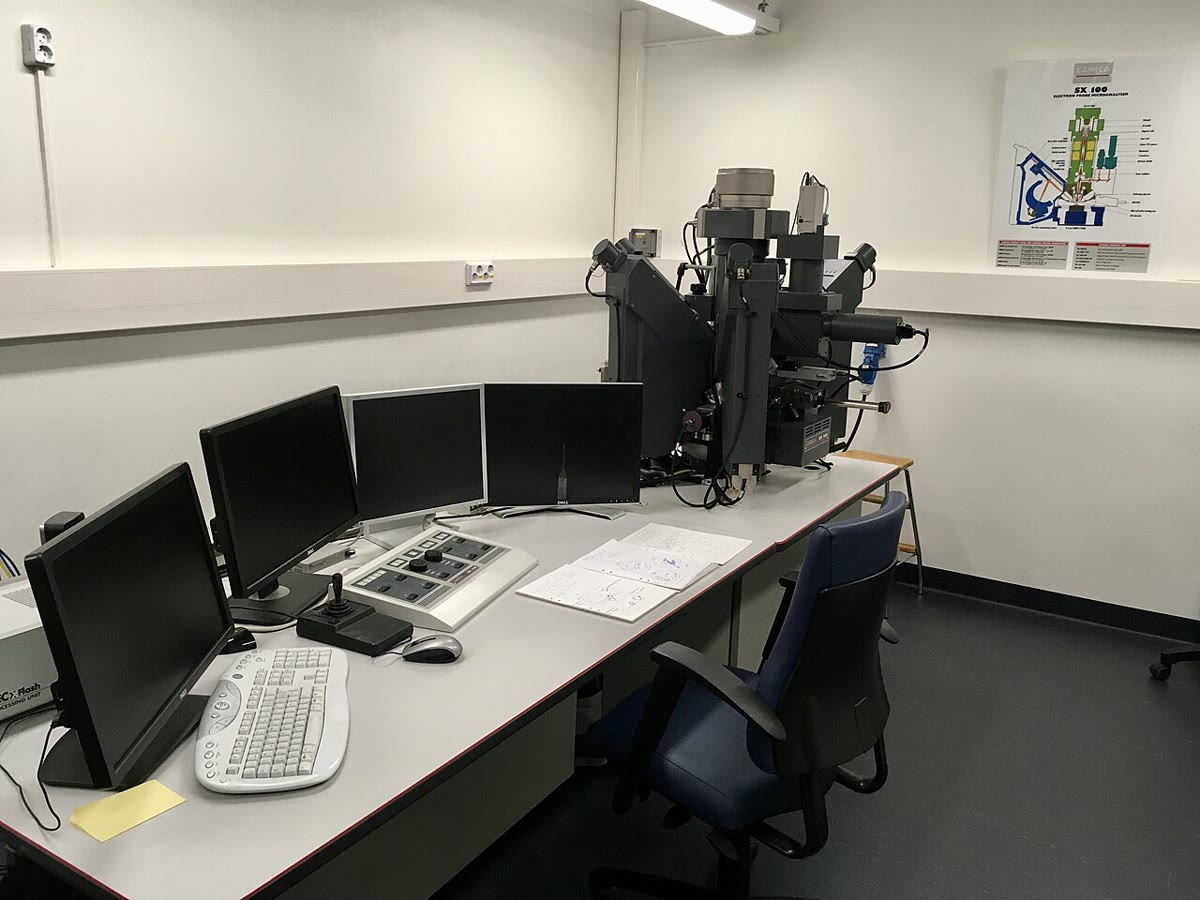
\includegraphics[width=\linewidth]{images/book4/b2-31-microprobe.jpg}
\par\smallskip{\scriptsize Een \omterm{def:b2:field-lab-methods-2:epma}{elektronenmicrosonde}: de elektronenkolom, met de spectrometers
eromheen, en de bedieningstafel. Foto Kallerna, CC BY-SA 4.0 (Wikimedia Commons).}
\end{minipage}
\end{inthelab}
% ledger: sercE:epma-spot, sercE:coating, photo:b2-31-microprobe

\section{Isotopenanalyse}\label{sec:b2:field-lab-methods-2:isotopes}

\omterm{def:b2:isotope-geochemistry:tracer}{Radiogene isotopentracers} en ouderdommen (\cref{ch:b2:isotope-geochemistry}) berusten op verhoudingen die gemeten zijn
tot op 0.01--\qty{0.001}{\percent}, aan elementen die van het gesteente zijn gescheiden door oplossing
en ionenwisselingschromatografie in een schoon laboratorium, met gefilterde lucht (doorgaans klasse 100 tot
1000), zodat stof niets toevoegt aan de kleine hoeveelheden die worden geanalyseerd.
% ledger: sercT:tims

\begin{definition}[Thermische-ionisatiemassaspectrometrie, multicollector-ICP-MS, massadiscriminatie]\label{def:b2:field-lab-methods-2:tims}
Bij \emph{thermische-ionisatiemassaspectrometrie}\index{thermische-ionisatiemassaspectrometrie} (TIMS) wordt een
gezuiverd element op een dun metalen lint aangebracht en geïoniseerd door het onder vacuüm te verhitten; de ionen
worden versneld over een potentiaal van tot \qty{10}{kV}, naar massa gescheiden in een magnetische sector
en opgevangen. Bij \emph{multicollector-ICP-MS}\index{multicollector-ICP-MS} komen de ionen uit een
inductief gekoppeld plasma, dat elementen ioniseert die thermisch moeilijk te ioniseren zijn, en meten verscheidene
collectoren de bundels van verschillende massa's tegelijk. De
\emph{massadiscriminatie}\index{massadiscriminatie} van een meting is de afwijking van een gemeten isotopenverhouding ten opzichte van de ware
verhouding van het monster, veroorzaakt door het instrument, dat de ene massa gemakkelijker doorlaat of ioniseert dan
de andere.
\end{definition}
% ledger: sercT:tims, sercM:mcicpms

Beide instrumenten bereiken deze precisie. TIMS ioniseert doorgaans minder dan
\qty{1}{\percent} van de atomen, en de \omterm{def:b2:field-lab-methods-2:tims}{massadiscriminatie} verandert voortdurend tijdens een meting. Ze wordt gecorrigeerd door de verhouding van twee isotopen vast te leggen die door geen
verval verandert, wat een element vraagt met minstens drie isotopen, waarvan twee stabiel en niet
radiogeen. Voor strontium wordt $^{86}\mathrm{Sr}/^{88}\mathrm{Sr}$ vastgelegd op 0.1194, en een gangbare
vorm van de correctie is de exponentiële wet.
% ledger: sercT:tims, sercM:mcicpms, cheong14:mass-bias, ciaaw:sr-isotopes

\begin{proposition}[Exponentiële wet van de massadiscriminatie]\label{prop:b2:field-lab-methods-2:bias}
Stel dat elke gemeten verhouding van twee isotopen met massa's $m_i$ en $m_j$ aan de ware
verhouding gekoppeld is door $R_{ij}^{\mathrm{true}} = R_{ij}^{\mathrm{meas}}\,(m_i/m_j)^{\beta}$, met één exponent
$\beta$ voor de hele meting. Dan geeft de gemeten verhouding $r$ van een referentiepaar, waarvan de ware waarde
$r_0$ bekend is,
\begin{equation}
\beta = \frac{\ln(r_0/r)}{\ln(m_k/m_l)}
\label{eq:b2:field-lab-methods-2:beta}
\end{equation}
voor het referentiepaar $k/l$, en wordt elke andere verhouding met dezelfde $\beta$ gecorrigeerd.
\end{proposition}

\begin{proof}
Toegepast op het referentiepaar luidt de wet $r_0 = r\,(m_k/m_l)^\beta$; logaritmen nemen geeft
$\ln(r_0/r) = \beta\ln(m_k/m_l)$, wat \eqref{eq:b2:field-lab-methods-2:beta} is. De exponent is
per hypothese gemeenschappelijk voor alle verhoudingen van de meting, zodat hij elk ervan corrigeert.
\end{proof}

Voor strontium is het referentiepaar $^{86}\mathrm{Sr}/^{88}\mathrm{Sr}$ met $r_0 = 0.1194$, en
de gecorrigeerde $^{87}\mathrm{Sr}/^{86}\mathrm{Sr}$ is de gemeten verhouding maal
$(m_{87}/m_{86})^\beta$. De CIAAW-abundanties, \qty{9.86}{\percent} strontium-86 en
\qty{82.58}{\percent} strontium-88, geven dezelfde waarde. Elke sessie meet ook een \omterm{def:b2:isotope-geochemistry:standards}{isotopische
referentiestandaard}: één laboratorium mat $^{87}\mathrm{Sr}/^{86}\mathrm{Sr} = 0.710252 \pm
0.000007$ op het referentiemateriaal NBS~987 in zeven metingen.
% ledger: cheong14:mass-bias, ciaaw:sr-isotopes

Verhoudingen alleen geven geen concentratie. Daarvoor wordt een bekende hoeveelheid van een \emph{spike}, een oplossing van
het element die kunstmatig verrijkt is in één isotoop, vóór de chemische scheiding met het opgeloste monster
gemengd, en wordt de verhouding in het mengsel gemeten. De TIMS-laboratoria gebruiken dit voor zowel
concentraties als verhoudingen tussen moeder- en dochterisotoop.
% ledger: sercT:tims

\begin{proposition}[Isotopenverdunning]\label{prop:b2:field-lab-methods-2:id}
Laat een monster $N_x$ mol van een referentie-isotoop $b$ bevatten en een spike $N_s$ mol ervan, en zij
$R_x$, $R_s$ en $R_m$ de verhoudingen van een tweede isotoop $a$ tot $b$ in het monster, de spike en
het mengsel. Dan geldt
\begin{equation}
N_x = N_s\,\frac{R_s - R_m}{R_m - R_x} .
\label{eq:b2:field-lab-methods-2:id}
\end{equation}
Een relatieve fout $\varepsilon$ op $R_m$ geeft $N_x$ de relatieve fout $\mathcal{M}\varepsilon$,
met de foutvergroting
\begin{equation}
\mathcal{M} = \frac{R_m\,(R_s - R_x)}{(R_s - R_m)(R_m - R_x)} ,
\label{eq:b2:field-lab-methods-2:mag}
\end{equation}
die het kleinst is wanneer $R_m = \sqrt{R_s R_x}$.
\end{proposition}
\index{isotopenverdunning}

\begin{proof}
Isotoop $a$ blijft bij het mengen behouden: $R_m(N_x + N_s) = R_x N_x + R_s N_s$, dus $N_x(R_m - R_x) =
N_s(R_s - R_m)$, wat \eqref{eq:b2:field-lab-methods-2:id} is. De logaritmische afgeleide ervan is
$\mathrm{d}\ln N_x/\mathrm{d}\ln R_m = R_m\,[-1/(R_s - R_m) - 1/(R_m - R_x)] = -\mathcal{M}$, met
$\mathcal{M}$ zoals in \eqref{eq:b2:field-lab-methods-2:mag}. Op de positieve constante $R_s - R_x$ na is
$1/\mathcal{M} = (R_s - R_m)(R_m - R_x)/R_m = R_s + R_x - R_m - R_sR_x/R_m$, waarvan de afgeleide
$-1 + R_sR_x/R_m^2$ nul wordt bij $R_m = \sqrt{R_sR_x}$, een maximum van $1/\mathcal{M}$.
\end{proof}

\omterm{prop:b2:field-lab-methods-2:id}{Isotopenverdunning} vraagt geen kalibratielijn en ook geen volledige terugwinning van het element tijdens
de chemische scheiding: zodra spike en monster gemengd zijn, treffen verliezen beide evenzeer. Een gepubliceerde
strontiumspike bevat bijvoorbeeld \qty{99.65}{\percent} strontium-84, met
$^{84}\mathrm{Sr}/^{88}\mathrm{Sr} = 561.4$ en $^{86}\mathrm{Sr}/^{88}\mathrm{Sr} = 0.7661$, bij
\qty{15.271}{\micro\gram} strontium per gram oplossing. Zijn verhouding 86/88 toont waarom de
\omterm{def:b2:field-lab-methods-2:tims}{massadiscriminatie} van een gespiket mengsel niet kan worden gecorrigeerd door $^{86}\mathrm{Sr}/^{88}\mathrm{Sr}$ op zijn
natuurlijke waarde vast te leggen: de spike heeft die verhouding verschoven.
% ledger: cheong14:spike, cheong14:mass-bias

\section{Een karteringscampagne op het venster van Varden}\label{sec:b2:field-lab-methods-2:campaign}

In de kern van de anticlinaal van Varden heeft de erosie de zandsteenbedekking doorsneden en de sokkel
blootgelegd: schist die door een graniet is geïntrudeerd. Een campagne die het laboratorium moet bevoorraden, begint in het
veld. Over het venster worden twee traverses van west naar oost gelopen, met een station om de
\qty{100}{m}; bij elk wordt de eenheid genoteerd, en worden verse monsters genomen waar het gesteente
onverweerd is, genummerd met het station, en, waar maaksels moeten worden gemeten, georiënteerd. De figuur
toont wat de stations tegenkomen: van de 30 liggen er tien op graniet, tien op de zandsteenbedekking, één op
de schist, één op kalksteen en acht op het alluvium van de dalbodem, waar geen gesteente
dagzoomt.

\begin{omfigure}
\centering
\begin{tikzpicture}
\begin{axis}[axis equal image, xmin=2.4, xmax=4.6, ymin=3.1, ymax=5.0, width=0.66\linewidth,
  tick label style={font=\scriptsize}, xlabel={oost (km)}, ylabel={noord (km)},
  label style={font=\small}]
% units: figdata/shared/region.py (read only); stations: figdata/bachelor-2/labmethods.py part stations
\addplot[lith schist, draw=black, line width=0.3pt, even odd rule] table {figdata/out/shared-region-unit-schist.dat};
\addplot[lith granite, draw=black, line width=0.3pt, even odd rule] table {figdata/out/shared-region-unit-granite.dat};
\addplot[om lith={icsTriassic!35}{om sand}, draw=black, line width=0.3pt, even odd rule] table {figdata/out/shared-region-unit-sandstone.dat};
\addplot[om lith={icsJurassic!40}{om limestone}, draw=black, line width=0.3pt, even odd rule] table {figdata/out/shared-region-unit-limestone.dat};
\addplot[om lith={icsJurassic!15}{om shale}, draw=black, line width=0.3pt, even odd rule] table {figdata/out/shared-region-unit-shale.dat};
\addplot[lith alluvium, draw=black, line width=0.3pt, even odd rule] table {figdata/out/shared-region-unit-alluvium.dat};
\addplot[river] table {figdata/out/shared-region-river.dat};
\addplot[only marks, mark=*, mark size=1.6pt, mark options={fill=white, draw=black}]
  table[x=x_km, y=y_km] {figdata/out/bachelor-2-labmethods-stations.dat};
\addplot[only marks, mark=*, mark size=1.6pt, mark options={fill=omThm, draw=black},
  x filter/.expression={\thisrow{unit}==2 ? x : nan}]
  table[x=x_km, y=y_km] {figdata/out/bachelor-2-labmethods-stations.dat};
\node[font=\scriptsize, fill=white, inner sep=1pt, anchor=east] at (axis cs:2.76,3.7) {1};
\node[font=\scriptsize, fill=white, inner sep=1pt, anchor=west] at (axis cs:4.24,3.7) {15};
\node[font=\scriptsize, fill=white, inner sep=1pt, anchor=east] at (axis cs:2.76,4.4) {16};
\node[font=\scriptsize, fill=white, inner sep=1pt, anchor=west] at (axis cs:4.24,4.4) {30};
\draw[black, line width=0.5pt] (axis cs:3.5,4.44) -- (axis cs:3.5,4.62);
\node[font=\scriptsize, fill=white, inner sep=1pt, anchor=south] at (axis cs:3.5,4.62) {station 23};
\pic at (axis cs:4.45,4.75) {northarrow};
\end{axis}
\end{tikzpicture}
\par\smallskip{\small Het sokkelvenster van de Varden Hills met de 30 stations van twee
traverses van west naar oost, \qty{100}{m} uit elkaar. Rode stippen: stations op graniet. Roze met kruisjes: graniet; grijs: schist; paars: zandsteen
uit het Trias; blauw: kalksteen uit het Jura; lichtblauw: schalie uit het Jura; crème: alluvium van de rivier, die
naar het oosten stroomt. Het
granietmonster van het weekendprobleem komt van station 23.}
\end{omfigure}

\begin{inthefield}[Bemonsteren voor het laboratorium]
\centering
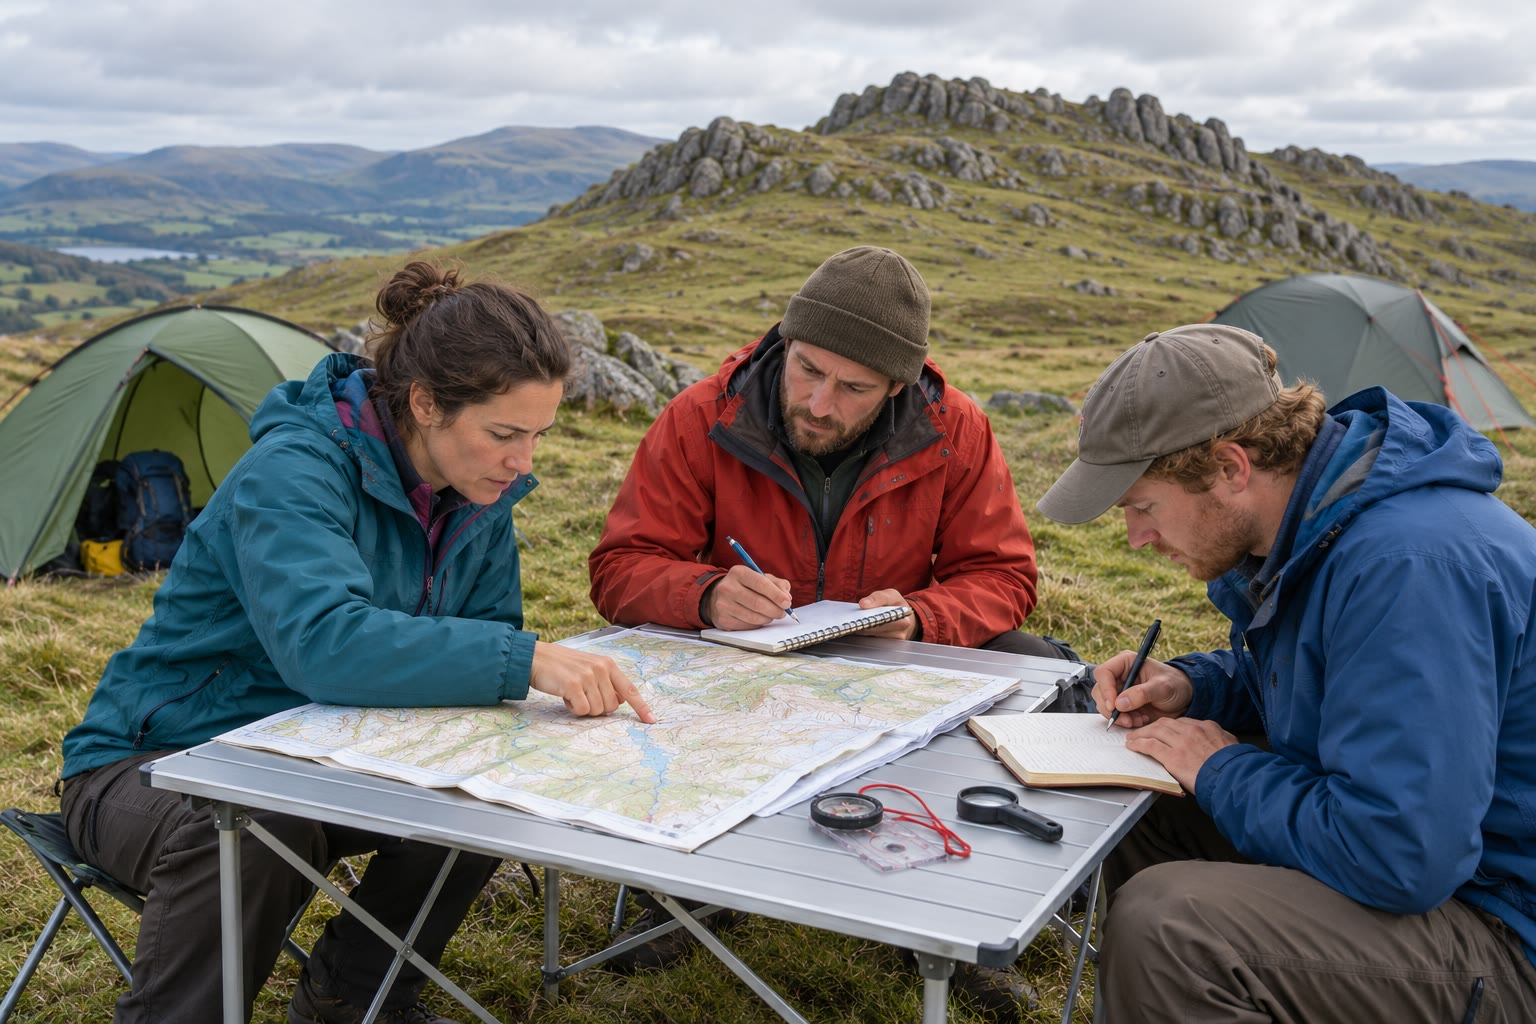
\includegraphics[width=0.56\linewidth]{images/book4/ai/b2-field-camp.jpg}
\par\smallskip{\small Een veldploeg plant de traverses van de volgende dag (door AI gegenereerde illustratie).}
\par\medskip\raggedright
's Avonds zet de ploeg de stations over op de kaart, controleert ze dat elk monsternummer in de
veldboeken bij een zak hoort, en beslist ze welke monsters naar welk laboratorium gaan. Eén monster van elke eenheid
gaat naar het slijplaboratorium; het meest verse graniet en de meest verse schist gaan
naar het breken en de analyse van het hele gesteente; enkele granietmonsters worden opzijgezet voor isotopen. Het
stationsnummer volgt elk monster door elke stap, van de zak naar het slijpplaatje, het
poeder, het tablet en de regel van een gegevenstabel, zodat elk vreemd resultaat kan worden herleid tot zijn
ontsluiting.
\end{inthefield}

\section{De kwaliteit van een getal}\label{sec:b2:field-lab-methods-2:quality}

Elke stap van de keten voegt zijn eigen fout toe, en de methoden van dit hoofdstuk tonen de twee soorten die
de scheikundeboeken onderscheiden. \omterm{def:b2:field-lab-methods-2:modal}{Puntentelling} en isotopenverhoudingen hebben vooral toevallige fouten, die
kleiner worden naarmate de tellingen groeien, als $1/\sqrt n$; kalibratie heeft systematische fouten, die herhaling niet
verkleint en die alleen een referentiemateriaal aan het licht brengt. De figuur van de silica-analyses toont
beide: de balken zijn de precisie van de methode, en een stip die nul mist met vele malen haar balk
gedeeld door de vierkantswortel van het aantal analyses, is een systematische afwijking. Hetzelfde element gemeten met twee
methoden, strontium door XRF en door \omterm{prop:b2:field-lab-methods-2:id}{isotopenverdunning}, is een extra controle, omdat de twee geen
kalibratie delen. Resultaten worden gerapporteerd met hun onzekerheid, daarop afgerond, en met de
referentiematerialen die ernaast zijn gemeten; een getal zonder die gegevens kan met geen enkel ander worden vergeleken.

\section*{Oefeningen}\label{sec:b2:field-lab-methods-2:exercises}

Gegevens voor de oefeningen, tenzij anders vermeld: atoommassa's H 1.008, O 15.999, Mg 24.305, Al
26.982, Si 28.085, K 39.098, Sr 87.62; isotopenmassa's $^{86}\mathrm{Sr}$ 85.909261,
$^{87}\mathrm{Sr}$ 86.908878, $^{88}\mathrm{Sr}$ 87.905612; natuurlijk strontium
$^{84}\mathrm{Sr}/^{86}\mathrm{Sr} = 0.05680$, \qty{9.86}{\percent} $^{86}\mathrm{Sr}$; de spike
uit de tekst, $^{84}\mathrm{Sr}/^{86}\mathrm{Sr} = 732.8$, \qty{0.13599}{\percent}
$^{86}\mathrm{Sr}$, atoomgewicht 83.9242, \qty{15.271}{\micro\gram\per\gram}. Rond af op drie
beduidende cijfers, tenzij anders vermeld.
% ledger: ciaaw:H, ciaaw:O, ciaaw:Mg, ciaaw:Al, ciaaw:Si, ciaaw:K, ciaaw:sr-isotopes, cheong14:spike

\begin{exercise}[$\star$]\label{exo:b2:field-lab-methods-2:1}
(a) Benoem de textuur of het kristal: (i) een doleriet waarin latten plagioklaas volledig zijn ingesloten in
grote augietkristallen; (ii) een marmer van even grote calcietkorrels waarvan de rechte grenzen per
drie samenkomen; (iii) een staurolietkristal van \qty{5}{mm} lang, vol kwartsinsluitsels, in een glimmerschist;
(iv) een granaat omringd door een doorlopende rand van plagioklaas en pyroxeen. (b) Drie korrelgrenzen
komen samen onder \ang{104}, \ang{128} en \ang{128}. Bepaal de verhouding van de spanning van de grens tegenover
de hoek van \ang{104} tot die van de andere.
\end{exercise}

\begin{exercise}[$\star$]\label{exo:b2:field-lab-methods-2:2}
Een grofkorrelig gesteente bevat \qty{25}{\percent} kwarts, 15 alkaliveldspaat, 40 plagioklaas, 12
biotiet en 8 hoornblende. (a) Herbereken Q, A en P. (b) Bepaal P/(A+P) en benoem het gesteente. (c) Bepaal
de kleurindex en kwalificeer het gesteente daarmee.
\end{exercise}

\begin{exercise}[$\star$]\label{exo:b2:field-lab-methods-2:3}
Een telling van 800 punten vindt een mineraal op \qty{12}{\percent}. (a) Bepaal de standaardafwijking van
dit aandeel, en de relatieve waarde ervan. (b) Hoeveel zou die bedragen met 3200 punten?
\end{exercise}

\begin{exercise}[$\star$]\label{exo:b2:field-lab-methods-2:4}
Een poeder van \qty{0.8000}{g} weegt \qty{0.7712}{g} na het gloeien, en het residu wordt gesmolten met
\qty{8.0000}{g} vloeimiddel. (a) Bepaal het \omterm{def:b2:field-lab-methods-2:xrf}{gloeiverlies}. (b) Bepaal de massafractie van het monster in
het tablet. (c) Het glas bevat \qty{5.20}{\percent} \ce{SiO2}. Bepaal het silicagehalte van het gegloeide poeder
en van het oorspronkelijke poeder.
\end{exercise}

\begin{exercise}[$\star\star$]\label{exo:b2:field-lab-methods-2:5}
(a) Hoeveel punten zijn nodig om een accessorisch mineraal dat \qty{2}{\percent} van een gesteente uitmaakt te meten
met een relatieve standaardfout van \qty{10}{\percent}? (b) En een mineraal dat \qty{30}{\percent} uitmaakt,
met dezelfde relatieve fout? (c) Geef commentaar op de inspanning die een zeldzaam mineraal vraagt.
\end{exercise}

\begin{exercise}[$\star\star$]\label{exo:b2:field-lab-methods-2:6}
In de USGS-resultaten van de figuur gaf de rhyoliet RGM-1 \ce{SiO2} $= 72.89$ met een
standaardafwijking van 0.19 in 20 analyses (aanbevolen 73.45), en het basalt BCR-2 54.17 met 0.13 in
20 analyses (aanbevolen 54.1). (a) Bepaal de terugwinning van elk, in procent. (b) Bepaal de
standaardafwijking van elk gemiddelde, en druk elk verschil met de aanbevolen waarde uit in eenheden daarvan.
(c) Welk resultaat vertoont een systematische afwijking? Is de methode minder precies voor RGM-1?
\end{exercise}

\begin{exercise}[$\star\star$]\label{exo:b2:field-lab-methods-2:7}
Een microsonde-analyse van een zuiver flogopiet, $\mathrm{KMg_3AlSi_3O_{10}(OH)_2}$, moet worden gecontroleerd.
(a) Bepaal de molaire massa van de formule en de massafractie \ce{H2O} die ze bevat. (b) Bepaal de
massafracties van \ce{K2O}, \ce{MgO}, \ce{Al2O3} en \ce{SiO2}, en het totaal dat een exacte analyse zou
geven. (c) Waarom is een totaal van ongeveer \qty{96}{\percent} voor een glimmer geen slechte analyse?
\end{exercise}

\begin{exercise}[$\star\star$]\label{exo:b2:field-lab-methods-2:8}
Een TIMS-meting op een strontiumstandaard geeft $^{86}\mathrm{Sr}/^{88}\mathrm{Sr} = 0.11905$ en
$^{87}\mathrm{Sr}/^{86}\mathrm{Sr} = 0.71062$. (a) Bepaal de exponent $\beta$ van de exponentiële wet.
(b) Corrigeer de verhouding $^{87}\mathrm{Sr}/^{86}\mathrm{Sr}$, op vijf decimalen. (c) Werd de lichte of
de zware isotoop bevoordeeld tijdens de meting?
\end{exercise}

\begin{exercise}[$\star\star$]\label{exo:b2:field-lab-methods-2:9}
Om zijn \omterm{prop:b2:field-lab-methods-2:id}{isotopenverdunning} te controleren, spiket een laboratorium \qty{0.0500}{g} van het referentiebasalt BHVO-2
met \qty{0.1000}{g} van de spike uit de tekst, en meet het $^{84}\mathrm{Sr}/^{86}\mathrm{Sr} =
0.874$ in het mengsel. (a) Bepaal het aantal mol $^{86}\mathrm{Sr}$ in de hoeveelheid spike. (b) Bepaal het
aantal mol $^{86}\mathrm{Sr}$ in het monster, en zijn strontiumconcentratie in ppm. (c) Vergelijk met
de aanbevolen \qty{394.1}{ppm}.
\end{exercise}

\begin{exercise}[$\star\star\star$]\label{exo:b2:field-lab-methods-2:10}
Voor de strontiumspike uit de tekst ($R_s = 732.8$, $R_x = 0.05680$): (a) bepaal de verhouding van het mengsel
die de foutvergroting minimaliseert, en de waarde ervan daar; (b) bereken $\mathcal M$ bij
$R_m = 0.1$, 0.5, 1.664 en 100; (c) leg uit waarom een mengsel dicht bij een van beide eindleden moet worden
vermeden, en hoeveel vrijheid de analist in de praktijk heeft.
\end{exercise}

\begin{exercise}[$\star\star\star$]\label{exo:b2:field-lab-methods-2:11}
Een telling in een graniet vindt 400 veldspaatpunten, waarvan \qty{62}{\percent} plagioklaas. (a) Behandel het
plagioklaas onder de veldspaatpunten als een binomiale telling en bepaal de standaardafwijking van
P/(A+P). (b) Hoe ver ligt het resultaat van de grens met granodioriet, in standaardafwijkingen? (c) Hoeveel
veldspaatpunten zouden het op twee standaardafwijkingen van de grens plaatsen?
\end{exercise}

\begin{exercise}[$\star\star\star$]\label{exo:b2:field-lab-methods-2:12}
Een mineraal neemt een fractie $p$ van een gesteente in. (a) Toon aan dat de kans dat $n$ onafhankelijke
punten het allemaal missen gelijk is aan $(1-p)^n$. (b) Hoeveel punten geven minstens \qty{95}{\percent} kans om
een mineraal dat \qty{1}{\percent} van het gesteente uitmaakt minstens één keer te raken? (c) Hetzelfde voor zirkoon met
\qty{0.05}{\percent}, en trek een conclusie over hoe naar een accessorisch mineraal moet worden gezocht.
\end{exercise}

\section*{Weekendprobleem}

\begin{problem}[{Weekendprobleem --- Van ontsluiting tot analyse}]\label{pb:b2:field-lab-methods-2:1}
% invented sample; data: ledger rows below; values: calc/ch31.py
Monster VH-23 van het graniet van Varden werd genomen bij station 23 van de campagne. Een slijpplaatje werd
geteld op een regelmatig raster van 1200 punten: kwarts 372, alkaliveldspaat 348, plagioklaas 324,
biotiet 108, muscoviet 36, opake oxiden 12. Een poeder van \qty{0.8000}{g} woog \qty{0.7949}{g}
na gloeien op \qty{925}{\celsius} en werd gesmolten met \qty{8.0000}{g} vloeimiddel. Tabletten van drie
referentiematerialen gaven deze \ce{SiO2}-intensiteiten (duizenden tellingen per seconde, kcps): BCR-2,
aanbevolen \qty{54.1}{\percent}, 21.66; AGV-2, 59.3, 23.70; RGM-1, 73.45, 29.37; het tablet van het graniet
gaf 28.63. De andere oxiden van het graniet tellen op tot \qty{27.15}{\percent}. Voor de isotopen werd
\qty{0.1000}{g} poeder opgelost en gemengd met \qty{0.2500}{g} van de spike uit de tekst;
het monster wordt geacht de natuurlijke strontiumabundanties van de oefeningen te hebben. Gebruik de gegevens van de
oefeningen.

\noindent\textbf{Deel I --- De modus.}
\begin{enumerate}
  \item Bepaal het modale aandeel van elk mineraal.
  \item Bepaal de standaardafwijking van het kwartsaandeel, en de relatieve standaardafwijking
        van het muscovietaandeel.
  \item Bepaal $M$ en de kleurindex $M'$, en kwalificeer het gesteente.
  \item Herbereken Q, A en P op een som van 100.
  \item Bepaal P/(A+P) en benoem het gesteente in het \omterm{def:b2:magmatic-series:qapf}{QAPF-diagram}.
  \item Is de naam zeker, gezien de binomiale standaardafwijking van P/(A+P) over de 672
        veldspaatpunten?
  \item Hoeveel punten zouden de standaardafwijking van het kwartsaandeel op één procentpunt
        brengen?
\end{enumerate}

\noindent\textbf{Deel II --- Silica door röntgenfluorescentie.}
\begin{enumerate}[resume]
  \item Bepaal het \omterm{def:b2:field-lab-methods-2:xrf}{gloeiverlies}.
  \item Bepaal de massafractie van het monster in het tablet, en het silicagehalte van het glas als het
        gegloeide poeder \qty{72}{\percent} bevat.
  \item Pas de kleinste-kwadratenlijn $c = aI + b$ aan door de drie referentiematerialen; geef $a$ op
        vier decimalen en $b$ op twee.
  \item Bepaal het \ce{SiO2}-gehalte van het graniet, op twee decimalen.
  \item Bepaal de residuen van de drie referentiematerialen. Is de lijn adequaat?
  \item Tel de oxiden en het \omterm{def:b2:field-lab-methods-2:xrf}{gloeiverlies} op. Zou de USGS-procedure deze analyse herhalen?
  \item Herbereken het silicagehalte op een som van 100 zonder de vluchtige bestanddelen.
\end{enumerate}

\noindent\textbf{Deel III --- Massadiscriminatie.}
\begin{enumerate}[resume]
  \item Bepaal uit de CIAAW-abundanties de natuurlijke $^{86}\mathrm{Sr}/^{88}\mathrm{Sr}$ en vergelijk
        met de waarde die voor de normalisatie wordt gebruikt.
  \item Een ongespiket deel geeft $^{86}\mathrm{Sr}/^{88}\mathrm{Sr} = 0.11853$. Bepaal $\beta$ op
        vier decimalen.
  \item Het geeft $^{87}\mathrm{Sr}/^{86}\mathrm{Sr} = 0.71655$. Corrigeer dit, op vijf decimalen.
  \item Bepaal de \omterm{def:b2:field-lab-methods-2:tims}{massadiscriminatie} per massa-eenheid, in procent.
  \item Waarom kan deze correctie niet worden uitgevoerd op het gespikete mengsel van Deel IV?
\end{enumerate}

\noindent\textbf{Deel IV --- Isotopenverdunning.}
\begin{enumerate}[resume]
  \item Controleer dat de spike \qty{99.65}{\percent} strontium-84 en \qty{0.13599}{\percent}
        strontium-86 bevat.
  \item Bepaal het aantal mol strontium en $^{86}\mathrm{Sr}$ in de hoeveelheid spike, op vier
        beduidende cijfers.
  \item Controleer de waarden $R_s = 732.8$ en $R_x = 0.05680$ van de oefeningen.
  \item De gecorrigeerde verhouding van het mengsel is $R_m = 1.6812$. Bepaal het aantal mol $^{86}\mathrm{Sr}$
        van het monster.
  \item Bepaal de foutvergroting. Bepaal, met $R_m$ bekend tot op \qty{0.01}{\percent} en de
        spikeconcentratie tot op $\pm\qty{0.031}{\micro\gram\per\gram}$, de relatieve onzekerheid van
        het resultaat.
  \item Bepaal de strontiumconcentratie van het graniet van Varden, in ppm.
\end{enumerate}
\end{problem}
% ledger: bgsI:qapf, bgsI:colour-index, usgsT:procedure, usgsT:sio2-table, ciaaw:sr-isotopes, cheong14:spike, cheong14:mass-bias
